\section{Retrieval with Synchronised Graph Expansion}
\label{sec:graph_retrieval}

\def\Tqinit{\mathbf{T}_\mathbf{q}}


\begin{figure}[thbp]
  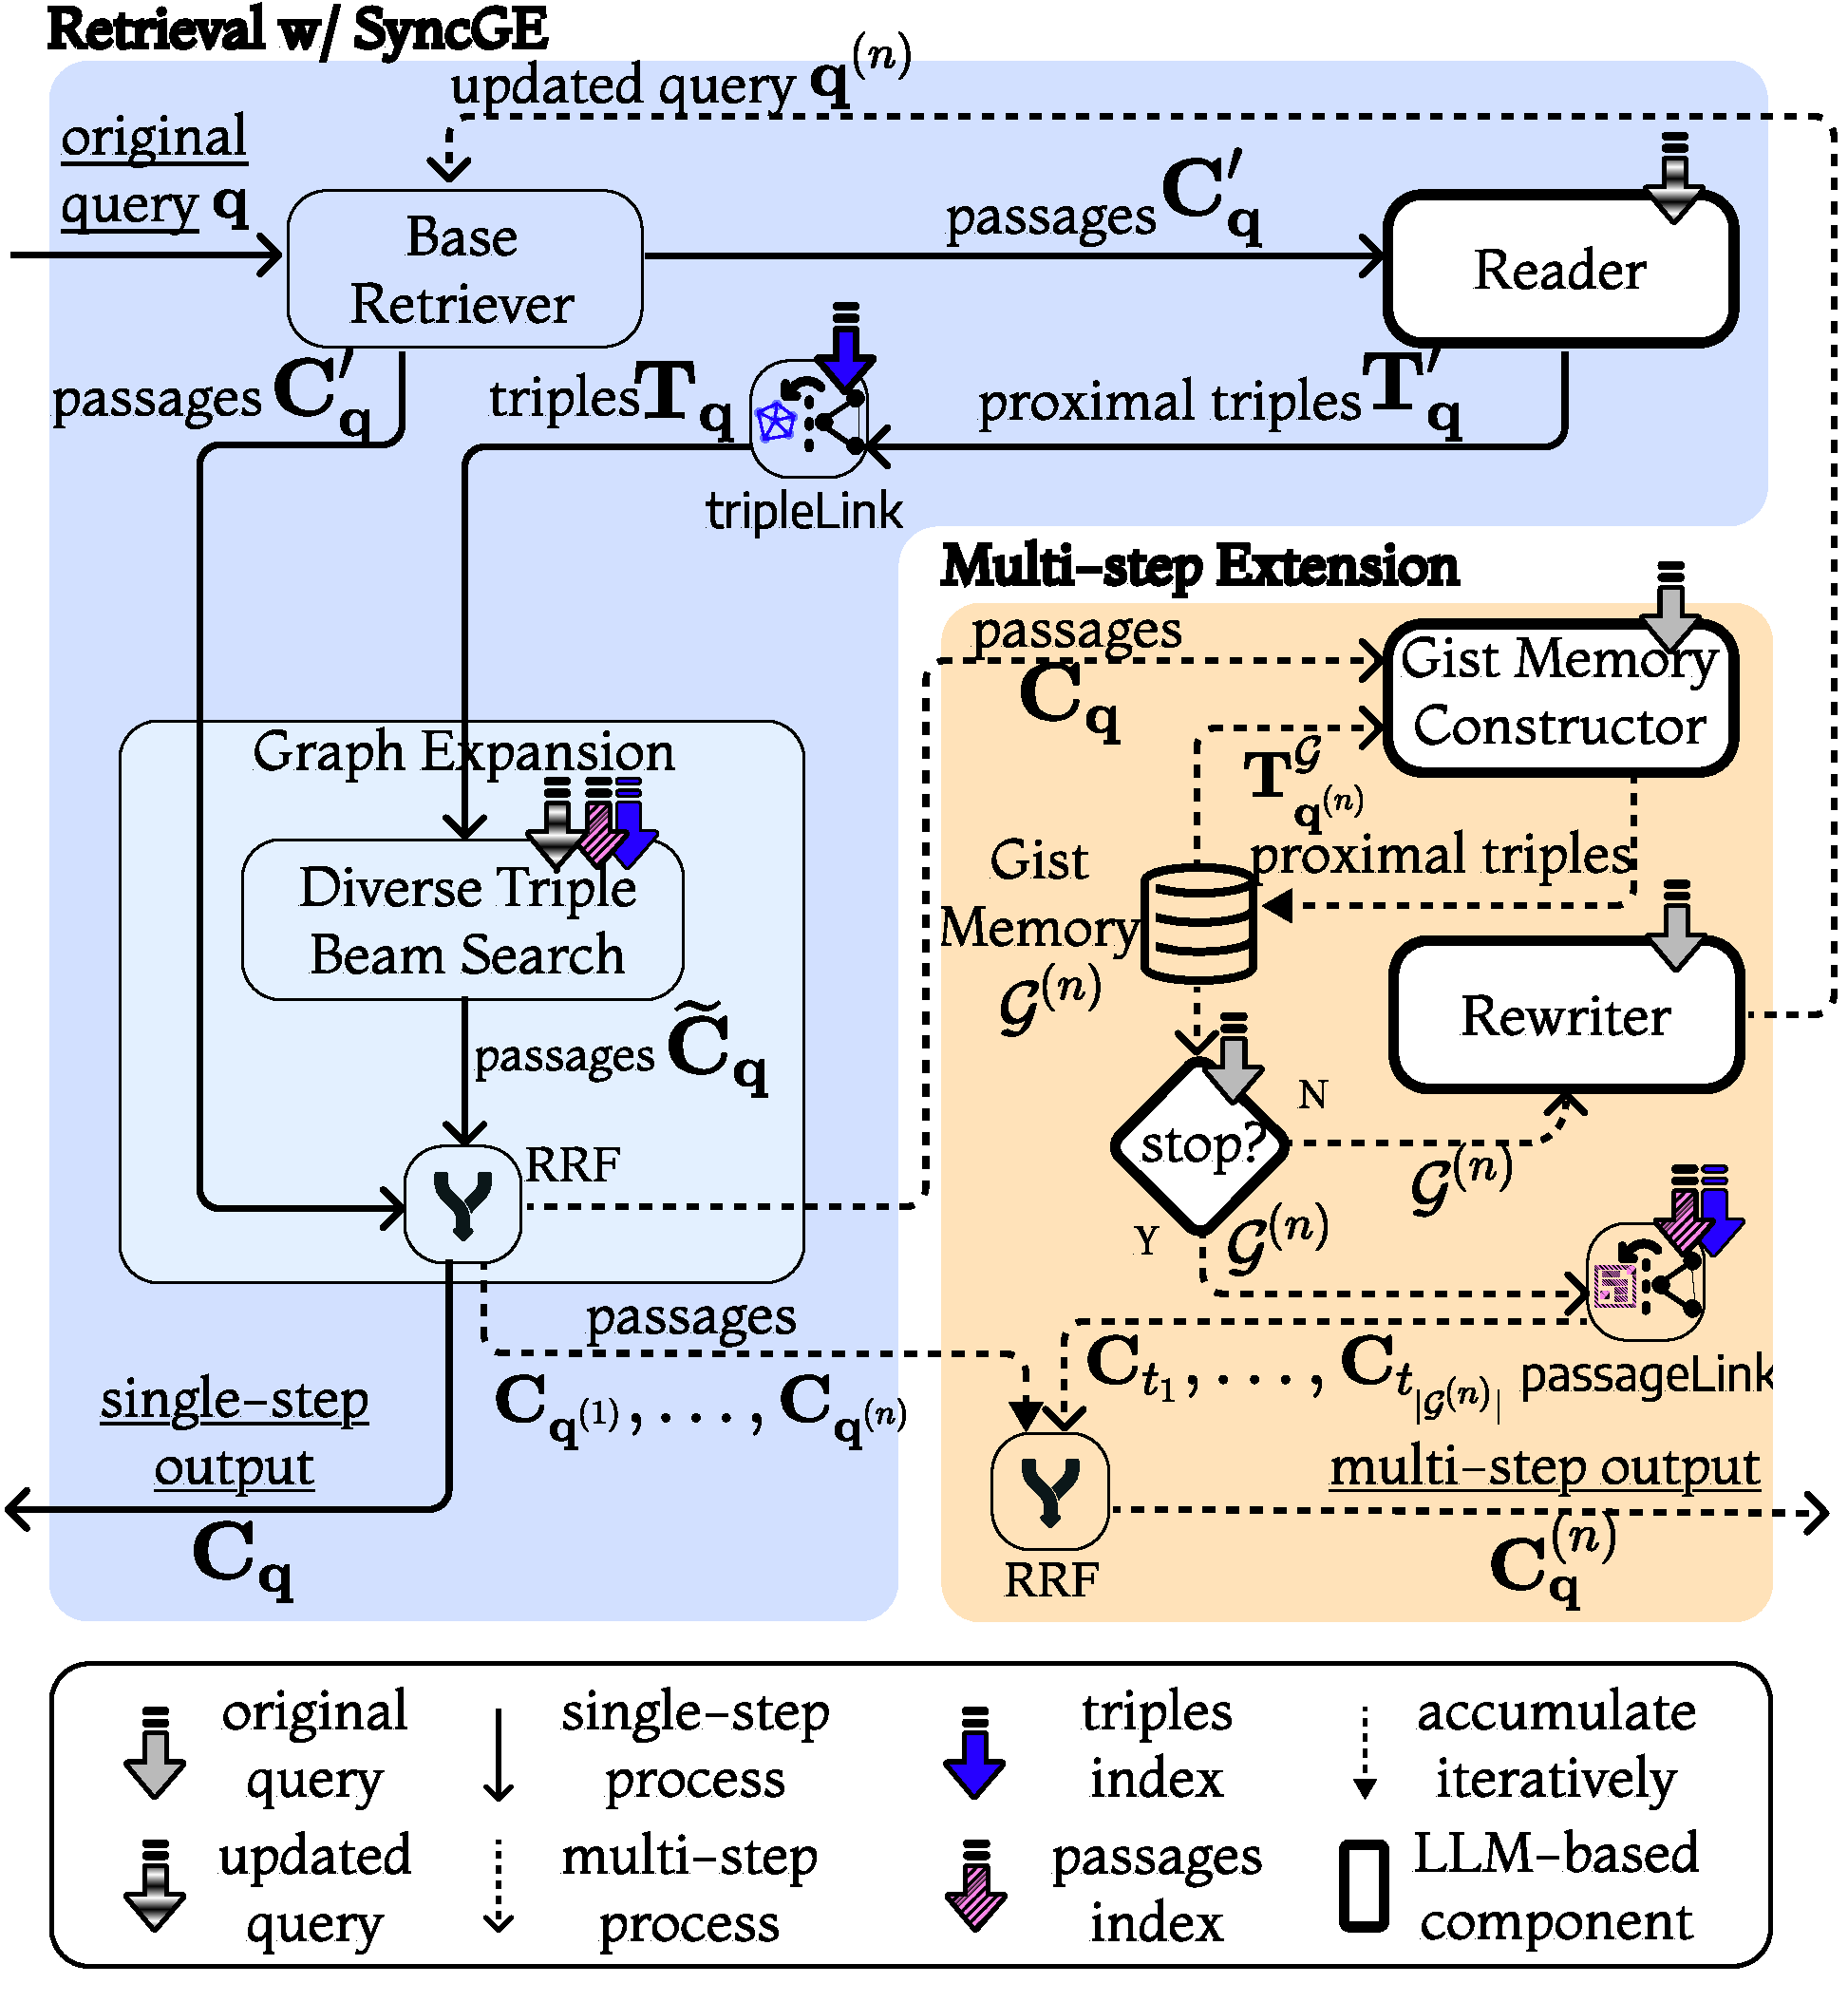
\includegraphics[width=\columnwidth]{figures/gear-sys-fig.pdf}
  \caption{\label{fig:system_diagram}System Architecture}
\end{figure}

% Start: Zhili --------------------------


Given an input query $\mathbf{q}$, let $\mathbf{C}_\mathbf{q}' = h^k_{\text{base}}\left( \mathbf{q}, {\mathbf{C}}\right )$  be a list of passages returned by the base retriever\footnote{The choice of a base retriever within our framework is flexible, without requiring any multi-hop capabilities.}.
Given this initially retrieved list of passages, $\mathbf{C}_\mathbf{q}'$, our goal is to derive relevant multi-hop contexts (passages) by retrieving a sub-graph of triples that interconnect their source passages. There are two challenges for materialising such sub-graph retrieval: \begin{inparaenum}[(i)]\item how to locate initial triples (i.e. starting nodes) $\Tqinit$, and \item how to expand the graph based on initial triples while reducing the search space\end{inparaenum}. The following sections address these challenges respectively, within \gear.



\subsection{Knowledge Synchronisation}
\label{subsection:knowledge_syncro}
\def\linkTriple{\texttt{tripleLink}}

We describe a knowledge \textbf{Sync}hronisation (\textbf{Sync}) process for locating initial nodes for graph expansion. We first employ an LLM to \texttt{read} $\mathbf{C}_\mathbf{q}'$ (see Appendix~\ref{subsec:online_retrieval_prompts}) and summarise knowledge triples that can support answering the current query $\mathbf{q}$, as defined:
\begin{align}
    \mathbf{T}_\mathbf{q}' = \texttt{read}\left (\mathbf{C}_\mathbf{q}', \mathbf{q}\right ).
    \label{eq:proximal_read}
\end{align}
$\mathbf{T}_\mathbf{q}'$ is a collection of triples to which we refer as \textit{proximal triples}. Initial nodes $\Tqinit$ for graph expansion can then be identified by linking each triple in $\mathbf{T}_\mathbf{q}'$ to a triple in $\mathbf{T}$, using the \linkTriple{} function:
\begin{align}
    \Tqinit =\left \{t_i | t_i = \linkTriple(t_i') ~ \forall t_i' \in \mathbf{T}_\mathbf{q}'\right \}.
\end{align}
The implementation of \linkTriple{} can vary. However, in this paper we consider it to be simply retrieving the most similar triple from $\mathbf{T}$.



\begin{algorithm}[ht]
\textbf{Input:} $\mathbf{q}$: query \\
\hspace*{3em} $b$: beam size \\
\hspace*{3em} $l$: maximum length \\
\hspace*{3em} $\mathrm{score}(\cdot, \cdot)$: scoring function \\
\hspace*{3em} $\{t_1, t_2, \ldots, t_n\}$: initial triples \\
\hspace*{3em} $\gamma$: hyperparameter for diversity


\begin{algorithmic}[1]
\State $B_0 \gets [\;]$
\For{$t \in \{t_1, t_2, ..., t_n\}$}
    \State $s \gets \mathrm{score}(\mathbf{q}, [t])$
    \State $B_0.\mathrm{add}(\langle s, [t] \rangle)$
\EndFor

\State $B_0 \gets \mathrm{top}(B_0, b)$


\For{$i \in \{1, \dots, l - 1\}$}
    \State $B \gets [\;]$
    
    \For{$\langle s, T \rangle \in B_{i-1}$}
        \State $V \gets [\;]$

        \For{$t \in \mathrm{get\_neighbours}(T.\mathrm{last}())$}
            \If{$\mathrm{exists}(t, B_{i-1})$}
                \State \textbf{continue}
            \EndIf
            
            \State $s' \gets s + \mathrm{score}(\mathbf{q}, T \circ t)$ ~ \texttt{\# concat} 
            \State $V.\mathrm{add}(\langle s', T \circ t \rangle)$
        \EndFor

        \State $\mathrm{sort}(V, \mathrm{descending})$

        \For{$n \in \{0, \dots, V.\mathrm{length()} - 1\}$}
            \State $\langle s', T \circ t \rangle \gets V[n]$
            \State $s' \gets s' \times e^{- \frac{\mathrm{min}(n, \gamma)}{\gamma}}$
            \State $B.\mathrm{add}(\langle s', T \circ t \rangle)$
        \EndFor
        
    \EndFor
    \State $B_i \gets \mathrm{top}(B, b)$
    
\EndFor

\State \Return $B_i$
\end{algorithmic}

\caption{Diverse Triple Beam Search}
\label{alg:beam_search}
\end{algorithm}

\subsection{Diverse Triple Beam Search}

We borrow the idea of constructing reasoning triple chains \cite{Fang2024} for expanding the graph, and present a retrieval algorithm: \textit{Diverse Triple Beam Search} (see Alg.~\ref{alg:beam_search}). 

We maintain top-$b$ sequences (beams) of triples and the scores at each step are determined by a scoring function. In this paper, we focus on leveraging a dense embedding model to compute the cosine similarity between embeddings of the query and a candidate sequence of triples, leaving other implementations of the scoring function for future work (see Section~\ref{sec:limitations}).

Considering all possible triple extensions at each step, in a Viterbi decoding fashion, would be intractable due to the size of $\mathbf{T}$. Consequently, we define the neighbourhood of a triple as the set of triples with shared head or tail entities (i.e. $\mathrm{get\_neighbours}$ in Alg.~\ref{alg:beam_search}). During each expansion step, we only consider neighbours of the last triple in the sequence, and avoid selecting previously visited triples (i.e. $\mathrm{exists}$ in Alg.~\ref{alg:beam_search}) to further reduce the search space.

While regular beam search can reduce the search space, it is prone to producing high-likelihood sequences that differ only slightly from one another \cite{Ippolito2019, Vijayakumar2018}. Our algorithm increases the diversity across beams to improve the recall for retrieval. In detail, for each beam, we sort candidate sequences extended from that beam in descending order, and weight their scores based on their relative positions. Candidate sequences that are ranked lower, within a beam, will receive smaller weights. Consequently, the resulting top-$b$ beams at each step are less likely to share the same starting sequence. 

The top-$b$ returned sequences are flattened in a breadth-first order. Each triple in the resulting list is then mapped to its source passage. This alignment between triples and passages is described in more detail in Section~\ref{sec:preliminaries}. Let $\widetilde{\mathbf{C}}_\mathbf{q}$ be the list of unique passages after alignment. The output of our graph expansion is then given by the Reciprocal Rank Fusion (RRF) \cite{Cormack2009} of $\widetilde{\mathbf{C}}_\mathbf{q}$ and the initial $\mathbf{C}_\mathbf{q}'$ list of passages :
\begin{align}
    \mathbf{C}_{\mathbf{q}} = \mathrm{RRF}\left(\widetilde{\mathbf{C}}_\mathbf{q}, \mathbf{C}_\mathbf{q}'\right ).
\end{align}
We refer to this graph-based method of retrieving relevant passages as \textbf{Sync}ronised \textbf{G}raph \textbf{E}xpansion (\textbf{SyncGE}).


\section{Multi-step Extension}


While SyncGE can enhance a base retriever with multi-hop context, some queries inherently require multiple steps to gather all necessary evidence. We materialise \gear by incorporating an agent with multi-turn capabilities, capable of interacting with the graph-retriever described above. We focus on:
\begin{itemize}
\item maintaining a gist memory of proximal knowledge obtained throughout the different steps 
\item incorporating a similar synchronisation process 
that summarises retrieved passages in proximal triples to be stored in this multi-turn gist memory
\item determining if additional steps are needed for answering the original input question
\end{itemize}
%
Within this multi-turn setting, the original input question $\mathbf{q}$ is iteratively decomposed into simpler queries: $\mathbf{q}^{(1)}, \ldots, \mathbf{q}^{(n)}$, where $\mathbf{q}^{(1)} = \mathbf{q}$ and $n \in \mathbb{N}$ represents the number of the current step.
For each query $\mathbf{q}^{(n)}$, we use the graph retrieval method introduced in Section~\ref{sec:graph_retrieval} in order to retrieve relevant passages $\mathbf{C}_{\mathbf{q}^{(n)}}$.



\subsection{Gist Memory Constructor}
To facilitate the multi-step capabilities of our agent, we introduce a \textit{gist memory}, $\mathcal{G}^{(n)}$, which is used for storing knowledge as an array of proximal triples. At the beginning of the first iteration, the gist memory is empty. During the $n$-th iteration, similar to the knowledge synchronisation module explained in Section~\ref{subsection:knowledge_syncro}, we employ an LLM to read a collection of retrieved paragraphs $\mathbf{C}_{\mathbf{q}^{(n)}}$ and summarise their content with proximal triples:

\begin{align}
\mathbf{T}_{\mathbf{q}^{(n)}}^{\mathcal{G}} = 
\begin{cases} 
    \texttt{read}\left(\mathbf{C}_{\mathbf{q}^{(n)}}, \mathbf{q} \right), & \text{if } n = 1 \\
    \texttt{read}\left(\mathbf{C}_{\mathbf{q}^{(n)}}, \mathbf{q}\textcolor{blue}{, \mathcal{G}^{(n-1)}} \right), & \text{if } n \geq 2
\end{cases}
\label{eq:proximal_read_agent}
\end{align}


Apart from the first iteration where Eq.~\ref{eq:proximal_read} and ~\ref{eq:proximal_read_agent} are identical, the inclusion of the memory in the \texttt{read} operation differentiates the construction of proximal triples produced at the subsequent steps compared to the ones from Eq.~\ref{eq:proximal_read}. $\mathcal{G}^{(n)}$ maintains the aggregated content of proximal triples s.t. 
\begin{align}
\mathcal{G}^{(n)} = \left[ \mathbf{T}_{\mathbf{q}^{(1)}}^{\mathcal{G}}  \circ \cdots \circ \mathbf{T}_{\mathbf{q}^{(n)}}^{\mathcal{G}} \right],
\end{align}where $\circ$ defines the concatenation operation. The triple memory serves as a concise representation of all the accumulated evidence, up to the $n$-th step. 

We believe the process introduced by the \texttt{read} step along with the information storage paradigm served by the gist memory, aligns well with the communication between the hippocampus and neocortex. The combination of the two establishes the synergetic behaviour between our graph retriever and the LLM that we seek to achieve within \gear.



\subsection{Reasoning for Termination}
After $\mathcal{G}^{(n)}$ is updated, we check the sufficiency of the accumulated evidence, within it, for answering the original question. This is achieved with the following LLM reasoning step:
\begin{align}
\mathbf{a}^{(n)}, \mathbf{r}^{(n)}   = \texttt{reason}(\mathcal{G}^{(n)}, \mathbf{q}),
\end{align}
% We can also call it 'sufficiency' instead of 'answerability'. I do not really have a preference.
where $\mathbf{a}^{(n)}$ denotes the query's answerability given the available evidence in $\mathcal{G}^{(n)}$, and $\mathbf{r}^{(n)}$ represents the reasoning behind this determination. When the query is deemed answerable, the system concludes its iterative process.



\subsection{Query Re-writing}
The query re-writing process leverages an LLM that incorporates three key inputs: the original query $\mathbf{q}$, the accumulated memory, and crucially, the reasoning output $\mathbf{r}^{(n)}$ from the previous step. This process can be formally expressed as:
\begin{align}
\mathbf{q}^{(n+1)} = \texttt{rewrite}\left (\mathcal{G}^{(n)}, \mathbf{q}, \mathbf{r}^{(n)} \right),
\end{align}
where $\mathbf{q}^{(n+1)}$ represents the updated query, which serves as input for the retriever in the next iteration.\\
\subsection{After Termination}
\gear aims to return a single ranked list of passages. Given the final gist memory $\mathcal{G}^{(n)}$ upon termination, we link each proximal triple in $\mathcal{G}^{(n)}$ to a list of passages as follows:
\begin{align}
    \mathbf{C}_{t_j} = \texttt{passageLink}\left(t_j, k\right),
\end{align}
where $j \in \left \{1, \dots, \vert\mathcal{G}^{(n)}\vert \right \}$. Similar to \texttt{tripleLink}, \texttt{passageLink} is implemented by retrieving passages with a triple as the query (see Appendix~\ref{appendixpara:passage_link}). The final list of passages returned by \gear is the RRF of the resulting linked passages and passages retrieved across iterations:
\begin{align}
\mathbf{C}_\mathbf{q}^{(n)} = \mathrm{RRF}\big(&\mathbf{C}_{t_1}, \ldots,\mathbf{C}_{t_{\vert\mathcal{G}^{(n)}\vert}}, \nonumber\\
    &\mathbf{C}_{\mathbf{q}^{(1)}}, \ldots, \mathbf{C}_{\mathbf{q}^{(n)}} \big).
\end{align}

All relevant prompts for the \texttt{read}, \texttt{reason} and \texttt{rewrite} steps are provided in Appendix~\ref{subsec:online_retrieval_prompts}.
